\ifx\allfiles\undefined
\documentclass[12pt, a4paper, oneside, UTF8]{ctexbook}
\def\path{../config}
\usepackage{amsmath}
\usepackage{amsthm}
\usepackage{amssymb}
\usepackage{array}
\usepackage{xcolor}
\usepackage{graphicx}
\usepackage{mathrsfs}
\usepackage{enumitem}
\usepackage{geometry}
\usepackage[colorlinks, linkcolor=black]{hyperref}
\usepackage{stackengine}
\usepackage{yhmath}
\usepackage{extarrows}
\usepackage{tikz}
\usepackage{pgfplots}
\usepackage{asymptote}
\usepackage{float}
\usepackage{fontspec} % 使用字体

\setmainfont{Times New Roman}
\setCJKmainfont{LXGWWenKai-Light}[
    SlantedFont=*
]

\everymath{\displaystyle}

\usepgfplotslibrary{polar}
\usepackage{subcaption}
\usetikzlibrary{decorations.pathreplacing, positioning}

\usepgfplotslibrary{fillbetween}
\pgfplotsset{compat=1.18}
% \usepackage{unicode-math}
\usepackage{esint}
\usepackage[most]{tcolorbox}

\usepackage{fancyhdr}
\usepackage[dvipsnames, svgnames]{xcolor}
\usepackage{listings}

\definecolor{mygreen}{rgb}{0,0.6,0}
\definecolor{mygray}{rgb}{0.5,0.5,0.5}
\definecolor{mymauve}{rgb}{0.58,0,0.82}
\definecolor{NavyBlue}{RGB}{0,0,128}
\definecolor{Rhodamine}{RGB}{255,0,255}
\definecolor{PineGreen}{RGB}{0,128,0}

\graphicspath{ {figures/},{../figures/}, {config/}, {../config/} }

\linespread{1.6}

\geometry{
    top=25.4mm, 
    bottom=25.4mm, 
    left=20mm, 
    right=20mm, 
    headheight=2.17cm, 
    headsep=4mm, 
    footskip=12mm
}

\setenumerate[1]{itemsep=5pt,partopsep=0pt,parsep=\parskip,topsep=5pt}
\setitemize[1]{itemsep=5pt,partopsep=0pt,parsep=\parskip,topsep=5pt}
\setdescription{itemsep=5pt,partopsep=0pt,parsep=\parskip,topsep=5pt}

\lstset{
    language=Mathematica,
    basicstyle=\tt,
    breaklines=true,
    keywordstyle=\bfseries\color{NavyBlue}, 
    emphstyle=\bfseries\color{Rhodamine},
    commentstyle=\itshape\color{black!50!white}, 
    stringstyle=\bfseries\color{PineGreen!90!black},
    columns=flexible,
    numbers=left,
    numberstyle=\footnotesize,
    frame=tb,
    breakatwhitespace=false,
} 

\lstset{
    language=TeX, % 设置语言为 TeX
    basicstyle=\ttfamily, % 使用等宽字体
    breaklines=true, % 自动换行
    keywordstyle=\bfseries\color{NavyBlue}, % 关键字样式
    emphstyle=\bfseries\color{Rhodamine}, % 强调样式
    commentstyle=\itshape\color{black!50!white}, % 注释样式
    stringstyle=\bfseries\color{PineGreen!90!black}, % 字符串样式
    columns=flexible, % 列的灵活性
    numbers=left, % 行号在左侧
    numberstyle=\footnotesize, % 行号字体大小
    frame=tb, % 顶部和底部边框
    breakatwhitespace=false % 不在空白处断行
}

% \begin{lstlisting}[language=TeX] ... \end{lstlisting}

% 定理环境设置
\usepackage[strict]{changepage} 
\usepackage{framed}

\definecolor{greenshade}{rgb}{0.90,1,0.92}
\definecolor{redshade}{rgb}{1.00,0.88,0.88}
\definecolor{brownshade}{rgb}{0.99,0.95,0.9}
\definecolor{lilacshade}{rgb}{0.95,0.93,0.98}
\definecolor{orangeshade}{rgb}{1.00,0.88,0.82}
\definecolor{lightblueshade}{rgb}{0.8,0.92,1}
\definecolor{purple}{rgb}{0.81,0.85,1}

\theoremstyle{definition}
\newtheorem{myDefn}{\indent Definition}[section]
\newtheorem{myLemma}{\indent Lemma}[section]
\newtheorem{myThm}[myLemma]{\indent Theorem}
\newtheorem{myCorollary}[myLemma]{\indent Corollary}
\newtheorem{myCriterion}[myLemma]{\indent Criterion}
\newtheorem*{myRemark}{\indent Remark}
\newtheorem{myProposition}{\indent Proposition}[section]

\newenvironment{formal}[2][]{%
	\def\FrameCommand{%
		\hspace{1pt}%
		{\color{#1}\vrule width 2pt}%
		{\color{#2}\vrule width 4pt}%
		\colorbox{#2}%
	}%
	\MakeFramed{\advance\hsize-\width\FrameRestore}%
	\noindent\hspace{-4.55pt}%
	\begin{adjustwidth}{}{7pt}\vspace{2pt}\vspace{2pt}}{%
		\vspace{2pt}\end{adjustwidth}\endMakeFramed%
}

\newenvironment{definition}{\vspace{-\baselineskip * 2 / 3}%
	\begin{formal}[Green]{greenshade}\vspace{-\baselineskip * 4 / 5}\begin{myDefn}}
	{\end{myDefn}\end{formal}\vspace{-\baselineskip * 2 / 3}}

\newenvironment{theorem}{\vspace{-\baselineskip * 2 / 3}%
	\begin{formal}[LightSkyBlue]{lightblueshade}\vspace{-\baselineskip * 4 / 5}\begin{myThm}}%
	{\end{myThm}\end{formal}\vspace{-\baselineskip * 2 / 3}}

\newenvironment{lemma}{\vspace{-\baselineskip * 2 / 3}%
	\begin{formal}[Plum]{lilacshade}\vspace{-\baselineskip * 4 / 5}\begin{myLemma}}%
	{\end{myLemma}\end{formal}\vspace{-\baselineskip * 2 / 3}}

\newenvironment{corollary}{\vspace{-\baselineskip * 2 / 3}%
	\begin{formal}[BurlyWood]{brownshade}\vspace{-\baselineskip * 4 / 5}\begin{myCorollary}}%
	{\end{myCorollary}\end{formal}\vspace{-\baselineskip * 2 / 3}}

\newenvironment{criterion}{\vspace{-\baselineskip * 2 / 3}%
	\begin{formal}[DarkOrange]{orangeshade}\vspace{-\baselineskip * 4 / 5}\begin{myCriterion}}%
	{\end{myCriterion}\end{formal}\vspace{-\baselineskip * 2 / 3}}
	

\newenvironment{remark}{\vspace{-\baselineskip * 2 / 3}%
	\begin{formal}[LightCoral]{redshade}\vspace{-\baselineskip * 4 / 5}\begin{myRemark}}%
	{\end{myRemark}\end{formal}\vspace{-\baselineskip * 2 / 3}}

\newenvironment{proposition}{\vspace{-\baselineskip * 2 / 3}%
	\begin{formal}[RoyalPurple]{purple}\vspace{-\baselineskip * 4 / 5}\begin{myProposition}}%
	{\end{myProposition}\end{formal}\vspace{-\baselineskip * 2 / 3}}


\newtheorem{example}{\indent \color{SeaGreen}{Example}}[section]
\renewcommand{\proofname}{\indent\textbf{\textcolor{TealBlue}{Proof}}}
\NewEnviron{solution}{%
	\begin{proof}[\indent\textbf{\textcolor{TealBlue}{Solution}}]%
		\color{blue}% 设置内容为蓝色
		\BODY% 插入环境内容
		\color{black}% 恢复默认颜色(可选,避免影响后续文字)
	\end{proof}%
}

% 自定义命令的文件

\def\d{\mathrm{d}}
\def\R{\mathbb{R}}
%\newcommand{\bs}[1]{\boldsymbol{#1}}
%\newcommand{\ora}[1]{\overrightarrow{#1}}
\newcommand{\myspace}[1]{\par\vspace{#1\baselineskip}}
\newcommand{\xrowht}[2][0]{\addstackgap[.5\dimexpr#2\relax]{\vphantom{#1}}}
\newenvironment{mycases}[1][1]{\linespread{#1} \selectfont \begin{cases}}{\end{cases}}
\newenvironment{myvmatrix}[1][1]{\linespread{#1} \selectfont \begin{vmatrix}}{\end{vmatrix}}
\newcommand{\tabincell}[2]{\begin{tabular}{@{}#1@{}}#2\end{tabular}}
\newcommand{\pll}{\kern 0.56em/\kern -0.8em /\kern 0.56em}
\newcommand{\dive}[1][F]{\mathrm{div}\;\boldsymbol{#1}}
\newcommand{\rotn}[1][A]{\mathrm{rot}\;\boldsymbol{#1}}

\newif\ifshowanswers
\showanswerstrue % 注释掉这行就不显示答案

% 定义答案环境
\newcommand{\answer}[1]{%
    \ifshowanswers
        #1%
    \fi
}

% 修改参数改变封面样式,0 默认原始封面、内置其他1、2、3种封面样式
\def\myIndex{0}


\ifnum\myIndex>0
    \input{\path/cover_package_\myIndex} 
\fi

\def\myTitle{考研数学笔记}
\def\myAuthor{Weary Bird}
\def\myDateCover{\today}
\def\myDateForeword{\today}
\def\myForeword{相见欢·林花谢了春红}
\def\myForewordText{
    林花谢了春红,太匆匆。
    无奈朝来寒雨晚来风。
    胭脂泪,相留醉,几时重。
    自是人生长恨水长东。
}
\def\mySubheading{以姜晓千强化课讲义为底本}


\begin{document}
% \input{\path/cover_text_\myIndex.tex}

\newpage
\thispagestyle{empty}
\begin{center}
    \Huge\textbf{\myForeword}
\end{center}
\myForewordText
\begin{flushright}
    \begin{tabular}{c}
        \myDateForeword
    \end{tabular}
\end{flushright}

\newpage
\pagestyle{plain}
\setcounter{page}{1}
\pagenumbering{Roman}
\tableofcontents

\newpage
\pagenumbering{arabic}
% \setcounter{chapter}{-1}
\setcounter{page}{1}

\pagestyle{fancy}
\fancyfoot[C]{\thepage}
\renewcommand{\headrulewidth}{0.4pt}
\renewcommand{\footrulewidth}{0pt}








\else
\fi
\chapter{操作系统}
\section{选择题}

\subsection{25-王道}
\begin{enumerate}
    \item 系统调用是由操作系统提供给用户的,它() \\
    A.直接通过键盘交互方式使用\qquad B.只能通过用户程序间接使用 \\
    C.是命令接口中的命令\qquad D.与系统的命令一样
    
    \item 操作系统与用户通信接口通常不包括() \\
    A.shell\qquad B.命令解释器\qquad C.广义指令\qquad D.缓存管理指令 

    \item 下列关于多道程序系统的叙述中,不正确的是() \\
    A.支持程序的并发执行\qquad B.不必支持虚拟存储管理 \\
    C.需要实现对共享资源的管理\qquad D.进程数越多CPU利用率也越多 

    \item 分时系统的一个重要指标是系统的响应时间,对操作系统的()因素改进有利于改善操作系统的响应时间. \\
    A.加大时间片\qquad B.采用静态页式管理 \\
    C.优先级+非抢占式调度算法\qquad D.代码可重入 

    \item 计算机区分内核态和用户态指令后,从核心态到用户态的转变用操作系统执行后完成,而用户态转换到核心态则有()完成 \\
    A. 硬件\qquad B.核心态程序\qquad C.用户程序\qquad D.中断处理程序

    \item "访管"指令()使用 \\
    A. 仅在用户态\qquad B.仅在内核态\qquad C.在规定时间内\qquad D.在调度时间内

    \item 在操作系统中,只能在核心态下执行的指令是() \\
    A. 读时钟\qquad B.取数\qquad C.广义指令\qquad D.寄存器清零

    \item \bt\bl 中断处理和子程序调用都需要压栈以保护现场,中断处理一定会保存而子程序调用不一定需要保存的内容是() \\
    A. 程序计数器\qquad B.程序状态字寄存器\qquad C.通用寄存器组\qquad D.通用地址寄存器

    \item \bt 定时器产生时钟中断后,由时钟中断服务程序更新的内容是()
    \begin{enumerate}
        \item [I] 内核中时间变量的值
        \item [II] 当前进程占用的CPU时间
        \item [III] 当前进程在时间片中的剩余执行时间
    \end{enumerate}
    A.仅I,II\qquad B.仅II,III\qquad C.仅I,III\qquad D.I,II,III

    \item \bt\bl 下列与中断相关的操作中,由操作系统完成的是(多选)()  
    \begin{enumerate}
        \item [I] 保存中断点
        \item [II] 提供中断服务
        \item [III] 初始化中断向量表
        \item [IV] 保存中断屏蔽字
    \end{enumerate}

    \item \bl 计算机的启动过程是(排序)() 
    \begin{enumerate}
        \item [1] CPU加点, CS:IP指向FFFF0H
        \item [2] 进行操作系统引导
        \item [3] 执行JMP指令跳转到BIOS
        \item [4] 登记BIOS中断例程入口地址
        \item [5] 硬件自检
    \end{enumerate}

    \item 在单处理机系统中,若同时存在10个进程,则处于就绪队列的进程最多有() \\
    A. 10个\qquad B.9个\qquad C.8个\qquad D.7个 

    \item 进程在处理器上执行时,() \\
    A. 进程之间是无关的,且具有封闭特性 \\
    B. 进程之间都有交互性,相互依赖,相互制约,具有并发性 \\
    C. 具有并发性,即同时执行的特性 \\
    D. 进程之间可能是无关的,但也可能是具有交互性的

    \item 在多对一的线程模型中,当一个多线程中的某线程被阻塞后() \\
    A. 该进程的其他线程仍然能够运行 \qquad B. 整个进程将被阻塞 \\
    C. 该阻塞进程将被撤销\qquad D. 该阻塞线程将永远不能再执行 

    \item 系统动态DLL库中的系统线程,被不同的进程所调用,它们是()的线程 \\
    A. 不同\qquad B.相同\qquad C.可能不同,可能相同\qquad D.不能被调用

    \item 下列不是多线程系统特长的是() \\
    A. 利用线程可以并发地执行矩阵乘法计算 \\
    B. Web服务器利用线程响应HTTP请求 \\
    C.键盘驱动程序为每个正在运行的程序配备一个线程,用以响应用户的输入 \\
    D. 基于GUI的调试程序用不同的线程分别处理用户输入,计算和跟踪等操作

    \item 下列选中,导致创建新进程的操作是(多选)() \\
    I.用户登录成功\qquad II.设备分配\qquad III,启动用户执行

    \item 可能导致进程被唤醒的事件是(多选)() \\
    I. I/O结束\qquad II.某进程退出临界区\qquad III.当前进程的时间片用完 

    \item 下列关于父进程与子进程的说法中错误的是() \\
    A.父进程和子进程可以并发执行 \\
    B.父进程和子进程共享虚拟地址空间 \\
    C.父进程和子进程有不同进程控制块 \\
    D.父进程和子进程共享临界资源

    \item 一个作业8:00到达系统,估计运行时间为1h,若10:00开始执行作业,其响应比为()

    \item 在进程调度算法中对短进程不利的是() \\
    A. 短进程优先调度\qquad B.先来先服务调度 \\
    C.高响应比优先调度算法\qquad D.多级反馈优先队列

    \item 不需要信号量就能实现的功能是() \\
    A.进程同步\qquad B.进程互斥\qquad C.进程的前驱关系\qquad D.进程的并发执行

    \item 若一个信号量的初始值为3,经过多次PV操作后当前值为-1,这表示进入临界区的进程数是() \\
    A. 1\qquad B.2\qquad C.3\qquad D.4

    \item 以下()属于临界资源 \\
    A. 打印机\qquad B.公用队列\qquad C.私有数据\qquad D.可重入的程序代码 

    \item 一个进程因在互斥信号量mutex上执行V操作而导致唤醒另一个进程的时,执行V操作后mutex的值为() \\
    A.大于0\qquad B.小于0\qquad C.大于等于0\qquad D.小于等于0 

    \item 进程P1和进程P2均包含并发执行的线程,部分伪代码如下,下列选项中,需要互斥执行的操作是() 
    \begin{center}
        \begin{minipage}[t]{0.45\textwidth}
\begin{lstlisting}[language=C]
// 进程P1                    
int x = 0;                   
Thread1() {                  
    int a;
    a = 1;
    x += 1;
}
Thread2() {
    int a;
    a = 2;
    x += 2;
}
\end{lstlisting}
        \end{minipage}
        \hfill
        \begin{minipage}[t]{0.45\textwidth}
\begin{lstlisting}[language=C]
// 进程P2                    
int x = 0;                   
Thread3() {                  
    int a;
    a = x;
    x += 3;
}
Thread4() {
    int a;
    b = x;
    x += 4;
}
\end{lstlisting}
        \end{minipage}
    \end{center}

    A.a=1与a=2\qquad B. a=x与b=x\qquad C.x +=1 与 x+=2\qquad D.x+=1与x+=3
    \item 下面是一个并发进程的程序代码,正确的是() 
    \begin{center}
        \begin{minipage}[t]{0.45\textwidth}
            \begin{lstlisting}[language=C]
Semaphore x1=x2=y=1;
int c1=c2=0;
P1() {
    while(1) {
        P(x1);
        if(++c1 == c) P(y);
        V(x1);
        computer(A);
        P(x1);
        if(--c1 == 0) V(y);
        V(x1);
    }
}
                \end{lstlisting}
            \end{minipage}
            \hfil
            \begin{minipage}[t]{0.45\textwidth}
                \begin{lstlisting}
Semaphore x1=x2=y=1;
int c1=c2=0;
P2() {
    while(1) {
        P(x2);
        if(++c2 == 1) P(y);
        V(x2);
        computer(B);
        P(x2);
        if(--c2 == 0) V(y);
        V(x2);
    }
}
            \end{lstlisting}
        \end{minipage}
    \end{center}
A.进程不会死锁,也不会饥饿 \qquad B.进程不会死锁,但会饥饿 \\
C.进程会死锁,但是不会饥饿\qquad D.进程会死锁,也会饥饿 

    \item 有两个并发进程,对于如这段程序的执行,正确的是() 
\begin{center}
    \begin{minipage}[t]{0.45\textwidth}
        \begin{lstlisting}
int x, y, z, t, u;
P1() {
    while(1) {
        x = 1;
        y = 0;
        if (x >= 1) y = y + 1;
        z = y;
    }
}
    \end{lstlisting}
\end{minipage}
\hfil
\begin{minipage}[t]{0.45\textwidth}
    \begin{lstlisting}
int x, y, z, t, u;
P2() {
    while(1) {
        x = 0;
        t = 0;
        if (x <= 1) t = t + 1;
        u = t;
    }
}
            \end{lstlisting}
        \end{minipage}
    \end{center}
    A.程序能够正常运行,结果唯一\qquad B.程序不能正常运行,可能出现两种结果\\
    C.程序不能正常运行,结果不确定\qquad D.程序不能正确运行,可能会死锁


    \item 若系统S1采用死锁避免方法,S2采用死锁检查方法,下列叙述中,正确的是(多选)() \\
    I. S1会限制用户申请资源的顺序,而S2不会 \\
    II. S1需要进程运行所需要的资源信息,而S2不需要 \\
    III. S1不会给可能导致死锁的进程分配资源,但S2会

    \item 下列存储管理方案中,()方式可以采用静态重定位 \\
    A.固定分区\qquad B.可变分区\qquad C.页式\qquad D.段式

    \item 下列不会产生内部碎片的存储管理是() \\
    A.分页式\qquad B.分段式\qquad C.段页式\qquad D.固定分区

    \item 采用分页和分段管理后,提供给用户的物理地址空间() \\
    A.分页支持更大的物理地址空间\qquad B.分段支持更大的物理地址空间 \\
    C.不能确定\qquad D.一样大

    \item 可重入程序是通过()方法来改善系统性能的. \\
    A.改变时间片长度\qquad B.改变用户数\qquad C.提供对换速度\qquad D.减少对换数量 

    \item 对主存储器的访问() \\
    A.以块(页)为单位 \qquad B.以字节或字位单位 \\
    C.随存储器的管理方案有所不同\qquad D.以用户的逻辑记录为单位

    \item 操作系统采用分页存储管理,要求() \\
    A.每个进程拥有一张页表,且进程的页表驻留在内存中 \\
    B.每个进程拥有一张页表,仅运行的进程的页表驻留在内存中\\
    C.所有进程共享一张页表,以节约有限的内存空间,但页表必须驻留在内存中 \\
    D.每个进程共享一张页表,只有页表中当前使用的页表必须驻留以最大限度节约有限的内存空间

    \item 在下列动态分区分配算法中,最容易产生内部碎片的是()  \\
    A.首次适应算法\qquad B.最坏适应算法\qquad C.最佳适应算法\qquad D.循环首次适应算法

    \item 请求分页存储管理中,若把页面尺寸增大一倍且可容纳的最大页数不变,则在程序顺序执行时缺页中断次数
    将会() \\
    A.增加\qquad B.减少\qquad C.不变\qquad D.无法确定

    \item 考虑页面置换算法,系统有m个物理块供调度,初始时全空,页面引用串长度为p,包含n个不同的页号,无论用啥算法
    缺页次数不会少于()

    \item 设主存容量为1MB,外存容量为400MB,计算机系统的地址寄存器有32位,那么虚拟存储器的最大容量是() 

    \item 导致LRU算法实现起来消耗特高的原因是() \\
    A.需要特殊硬件支持\qquad B.需要特殊的中断处理程序 \\
    C.需要在页表中标明特殊的页类型\qquad D.需要对所有页进行排序

    \item 在页面置换策略中,()策略可能引起抖动. 
    \begin{choices}
        \task FIFO
        \task LRU
        \task 没有一种 
        \task 所有 
    \end{choices}

    \item 提供虚拟存储技术的存储管理方法右() 
    \begin{choices}[2]
        \task 动态分区存储管理
        \task 页式存储管理
        \task 请求段式存储管理
        \task 存储覆盖技术
    \end{choices}

    \item 下列说法中正确的是() 
    \begin{enumerate}
        \item [(1)] 先进先出页面置换算法会产生Belady现象
        \item [(2)] 最近最少使用算法会产生Belady现象
        \item [(3)] 在进程运行时,若其工作集页面都在虚拟存储器内,则能够使该进程有效地进行,否则
        会频繁的页面调入/调出
        \item [(4)] 在进程运行时,若其工作集页面都在主存储器内,则能够使该进程有效地进行,否则
        会频繁的页面调入/调出
    \end{enumerate}
    \begin{choices}
        \task 1,3
        \task 1,4
        \task 2,3
        \task 2,4
    \end{choices}

    \item \bl 系统为某进程分配了4个页框,该进程已访问的页号序列为\underline{2,0,2,9,3,4,2,8,2,4,8.4.5}.
    若进程要访问的下一页的页号为7,依据LRU算法,应淘汰的页号是(   ) 

\end{enumerate}

\subsection{强化-1000题}
\begin{enumerate}
    \item 关于I/O接口的I/O逻辑说法错误的是(\qquad)
    \begin{choices}[1]
    \task 不同I/O接口的I/O端口不重复,各I/O逻辑同时对地址线上的地址进行译码,分辨出此次传输是否属于自己
    \task 通过控制线的读/写信号来对地址标明的I/O端口进行读写
    \task 对控制寄存器的I/O命令字进行译码,对外设发出具体的控制
    \task 采集外设的状态,并通过控制线向CPU反馈设备状态信息以及发出中断请求
    \end{choices}

    \item 在下列关于各种I/O控制方式的说法中,错误的是(\qquad)
    \begin{choices}[1]
    \task 程序直接控制I/O方式适用于结构简单、只需少量硬件的电路,不需要设备驱动程序来完成数据的传输工作
    \task 中断驱动I/O方式适用于具有中断机构的系统,用于处理中低速的I/O操作和随机事件
    \task DMA方式适用于具有DMA控制器的系统,用于高速外设的大批量数据传输
    \task 设备驱动程序和各种I/O控制方式之间密切相关
    \end{choices}

    \item 键盘硬件产生输入后,系统的正确处理流程是(\qquad)
    \begin{choices}[1]
    \task 键盘硬件→中断处理程序→设备驱动程序→进程调度→系统调用返回→用户程序
    \task 键盘硬件→设备驱动程序→中断处理程序→系统调用返回→进程调度→用户程序
    \task 键盘硬件→系统调用返回→设备驱动程序→中断处理程序→进程调度→用户程序
    \task 键盘硬件→中断处理程序→系统调用返回→设备驱动程序→进程调度→用户程序
    \end{choices}

    \item 用户进程调用了读磁盘系统调用,其中将逻辑盘块号转换为物理地址的工作是由(\qquad)完成的
    \begin{choices}
    \task 设备无关软件
    \task 设备驱动程序
    \task 中断处理程序
    \task 硬件
    \end{choices}

    \item 以下设备管理工作中,适合由设备独立性软件来完成的有(\qquad)\\
    I.向控制寄存器写命令\quad
    II.检查用户是否有权使用设备\quad
    III.检查用户I/O请求的合法性\quad
    IV.缓冲管理
    \begin{choices}[2]
    \task I、II、III
    \task II、III、IV
    \task II、IV
    \task I、II、III、IV
    \end{choices}

    \item 设备分配策略与(\qquad)因素有关\\
    I.I/O设备的固有属性\quad
    II.系统所采用的分配策略\quad
    III.设备分配中的安全性\quad
    IV.设备的无关性
    \begin{choices}[2]
    \task I、II、III
    \task I、III、IV
    \task I、II、IV
    \task I、II、III、IV
    \end{choices}

    \item 设备分配策略的主要目标是(\qquad)\\
    I.确保设备不被过度使用\quad
    II.提高设备利用率\quad
    III.减少用户等待时间
    \begin{choices}[2]
    \task I、II
    \task I、III
    \task II、III
    \task I、II、III
    \end{choices}

    \item 在设备分配与回收过程中,计算机需要访问的数据结构有:设备控制表DCT、控制器控制表COCT、通道控制表CHCT和系统设备表SDT,它们在设备分配流程中访问的先后顺序为(\qquad)
    \begin{choices}[2]
    \task DCT→COCT→CHCT→SDT
    \task SDT→DCT→COCT→CHCT
    \task SDT→COCT→CHCT→DCT
    \task DCT→COCT→SDT→CHCT
    \end{choices}

    \item 若某系统采用了SPOOLing技术,则用户进程打印的数据首先被传送到(\qquad)
    \begin{choices}
    \task 输出井
    \task 输入井
    \task 内存
    \task 外部设备
    \end{choices}

    \item 下列关于虚拟设备的说法中,正确的是(\qquad)
    \begin{choices}[1]
    \task 虚拟设备是指允许用户以统一的接口使用物理设备
    \task 虚拟设备是指允许用户使用比系统具有的物理设备更多的设备
    \task 虚拟设备是指把一个物理设备变换为多个对应的逻辑设备
    \task 虚拟设备是指允许用户程序部分装入内存即可使用系统中的设备
    \end{choices}

    \item 下面不属于设备驱动程序的功能的是(\qquad)
    \begin{choices}[1]
    \task 访问I/O端口,向外部设备发送读写命令
    \task 提供上层系统所需的I/O设备操作接口,隐藏具体的操作细节
    \task 查询设备状态并返回给上层系统
    \task 为I/O设备提供缓冲区,加速I/O
    \end{choices}

    \item 关于进程A执行“scanf函数”的说法正确的是(\qquad)
    \begin{choices}[1]
    \task 唤醒进程A由对应的系统调用服务例程完成
    \task 将数据从寄存器送往内核缓冲区由系统调用服务程序完成
    \task 将数据从内核缓冲区送往用户缓冲区由中断服务程序完成
    \task 初始化键盘设备的代码在驱动程序中
    \end{choices}

    \item 下列关于磁盘的说法中正确的有(\qquad)\\
    I.磁盘地址构成为:柱面号—磁道号—扇区号\quad
    II.磁盘驱动器是CPU与磁盘设备之间的I/O接口\quad
    III.磁盘逻辑格式化时,完成对磁盘的分区(如Windows系统中的C盘、D盘)
    \begin{choices}[2]
    \task 仅II
    \task I、II
    \task I、III
    \task 全部错误
    \end{choices}

    \item 下列关于磁盘调度的说法中,正确的有(\qquad)\\
    I.一次磁盘读/写操作中,寻道时间占大头\quad
    II.FCFS算法会导致磁臂粘着\quad
    III.将磁盘替换为随机访问的Flash半导体存储器后,FCFS调度策略效率最高
    \begin{choices}[2]
    \task 仅I
    \task 仅I、II
    \task 仅I、III
    \task I、II、III
    \end{choices}

    \item 某磁盘共200个磁道,编号从0到199现有一个磁盘请求序列为:142,82,197,90,108,当前磁头的位置为100,正在向磁道号增加的方向移动则按照最短寻道时间优先算法(SSTF)和改进后的SCAN扫描算法(LOOK),处理完以上请求后,磁头扫过的磁道数分别为(\qquad)
    \begin{choices}
    \task 149,212
    \task 149,216
    \task 342,212
    \task 342,216
    \end{choices}

    \item 已知磁道号从0到99,假设当前磁头位置为78号磁道,且正向磁道号增大的方向移动现有一个磁盘读写请求队列为:65,34,24,89,86,53,74,98若采用CLOOK算法依次响应这些请求,则平均移动的磁道数是
    \begin{choices}
    \task 16
    \task 17
    \task 18
    \task 19
    \end{choices}

    \item 某磁盘组共有80个柱面,每个柱面有12条磁道,每条磁道划分为16个扇区,现有一个8000条逻辑记录的文件,逻辑记录的大小与扇区大小相等,该文件按顺序结构存放在磁盘组上,柱面、磁道、扇区均从0开始编址,逻辑记录的编号从0开始,文件数据从0号柱面、0号磁道、0号扇区开始存放,则该文件的5687号逻辑记录应存放在(\qquad)
    \begin{choices}
    \task 29号柱面,7号磁道,6号扇区
    \task 30号柱面,8号磁道,7号扇区
    \task 29号柱面,7号磁道,7号扇区
    \task 28号柱面,7号磁道,7号扇区
    \end{choices}

    \item 下列关于固态硬盘(SSD)的说法中,错误的是(\qquad)
    \begin{choices}[1]
    \task 固态硬盘不受震动和物理冲击的影响,更适合移动设备使用
    \task 固态硬盘的磨损均衡技术中,动态磨损均衡比静态磨损均衡技术更先进、表现更优秀
    \task 固态硬盘的数据存储于Flash芯片之中
    \task 机械硬盘使用的硬盘调度算法不一定适用于固态硬盘
    \end{choices}

    \item 下列关于固态硬盘SSD的说法中,正确的有(\qquad)\\
    I.固态磁盘是基于闪存技术的存储技术\quad
    II.固态磁盘在写入前必须进行擦除\quad
    III.固态磁盘的读写性能、使用寿命均优于机械硬盘\quad
    IV.固态硬盘写入时,总是要选择擦写次数少的存储块
    \begin{choices}[2]
    \task I、II
    \task I、II、III
    \task I、II、IV
    \task II、III、IV
    \end{choices}

    \item 检查用户是否有权使用设备是在I/O软件的(\qquad)完成的.
    \item 判断正误
    \begin{choices}[1]
        \task 设备驱动程序应该允许系统调用
        \task 引入缓冲区可以减少I/O中断的频率,放宽CPU中断响应时间的限制
        \task SPOOLing技术用时间换空间
    \end{choices}

    \item 信息在外存空间的排序也会影响存取等待时间.考虑几条逻辑记录A,B,C,....,J.它们被存放于磁盘上,
    每个磁道存放10条记录,安排如表第一行所示,假定要经常按顺序处理这些记录,磁道旋转速度为20ms/转,处理程序读出每条记录后
    花4ms进行处理.考虑对信息进行优化,优化后如表第二列所示,相比于之前的信息分布,优化后的时间缩短了(\qquad)
    \begin{center}
    \begin{tabular}{|c|c|c|c|c|c|c|c|c|c|c|}
    \hline
    \textbf{物理块} & 1 & 2 & 3 & 4 & 5 & 6 & 7 & 8 & 9 & 10 \\ \hline 
    \textbf{逻辑记录(未优化)} & A & B & C & D & E & F & G & H & I & J \\ \hline 
    \textbf{逻辑记录(优化后)} & A & H & E & B & I & F & C & J & G & D \\ \hline 
    \end{tabular}
    \end{center}
    
    \item 一个交叉存放信息的磁盘,信息存放方式如图所示.每个磁道有8个扇区,每个扇区大小为512B,旋转速度为3000r/min
    假定磁头已在读取信息的磁道上,0扇区转到磁头下需要1/2转,且设备对应的控制器不能同时进行输入/输出,在数据从控制器传送至内
    存的这段时间内,从磁头下通过的扇区数为2.问依次读取一个磁道上所有扇区的数据到内存的平均传输速度为(\qquad)
    \begin{center}
    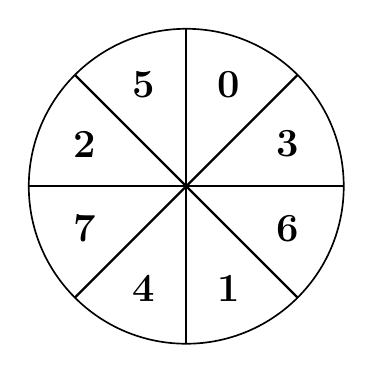
\begin{tikzpicture}
        \def\R{2cm}          
        \def\list{0,3,6,1,4,7,2,5}  
        \draw[line width=.6pt] (0,0) circle (\R);
        \foreach \idx [count=\i from 0] in \list{
            \draw[thick] (0,0) -- ++(90-\i*45:\R);
            \node at (90-\i*45-22.5:0.7*\R) {\Large\bfseries \idx};
        }
    \end{tikzpicture}
    \end{center}
\end{enumerate}
\ifx\allfiles\undefined
\end{document}
\fi